\pack~aims to facilitate the implementation of statistical methods described in \citet{riviere_hierarchical_2015} and \citet{riviere_hierarchical_2015-1}.
These methods aim to analyse highly unbalanced datasets that can be found in decentralized participatory plant breeding (PPB).

It has been developped for dataset with two types of farms, regional and satellite, based on their experimental design.

Regional farms had several populations (i.e. a germplasm in an environment) in two or more blocks with populations replicated in each block.
Satellite farms had no block and one germplasm replicated twice.
Farmers chose the other populations to be sown that were not replicated (Figure \ref{plan_SF_RF}).
The number of populations may vary between farms.

\begin{figure}[H]
        \begin{center}
                \begin{tabular}{|m{.25\textwidth}|m{.45\textwidth}|}
                        \hline
                        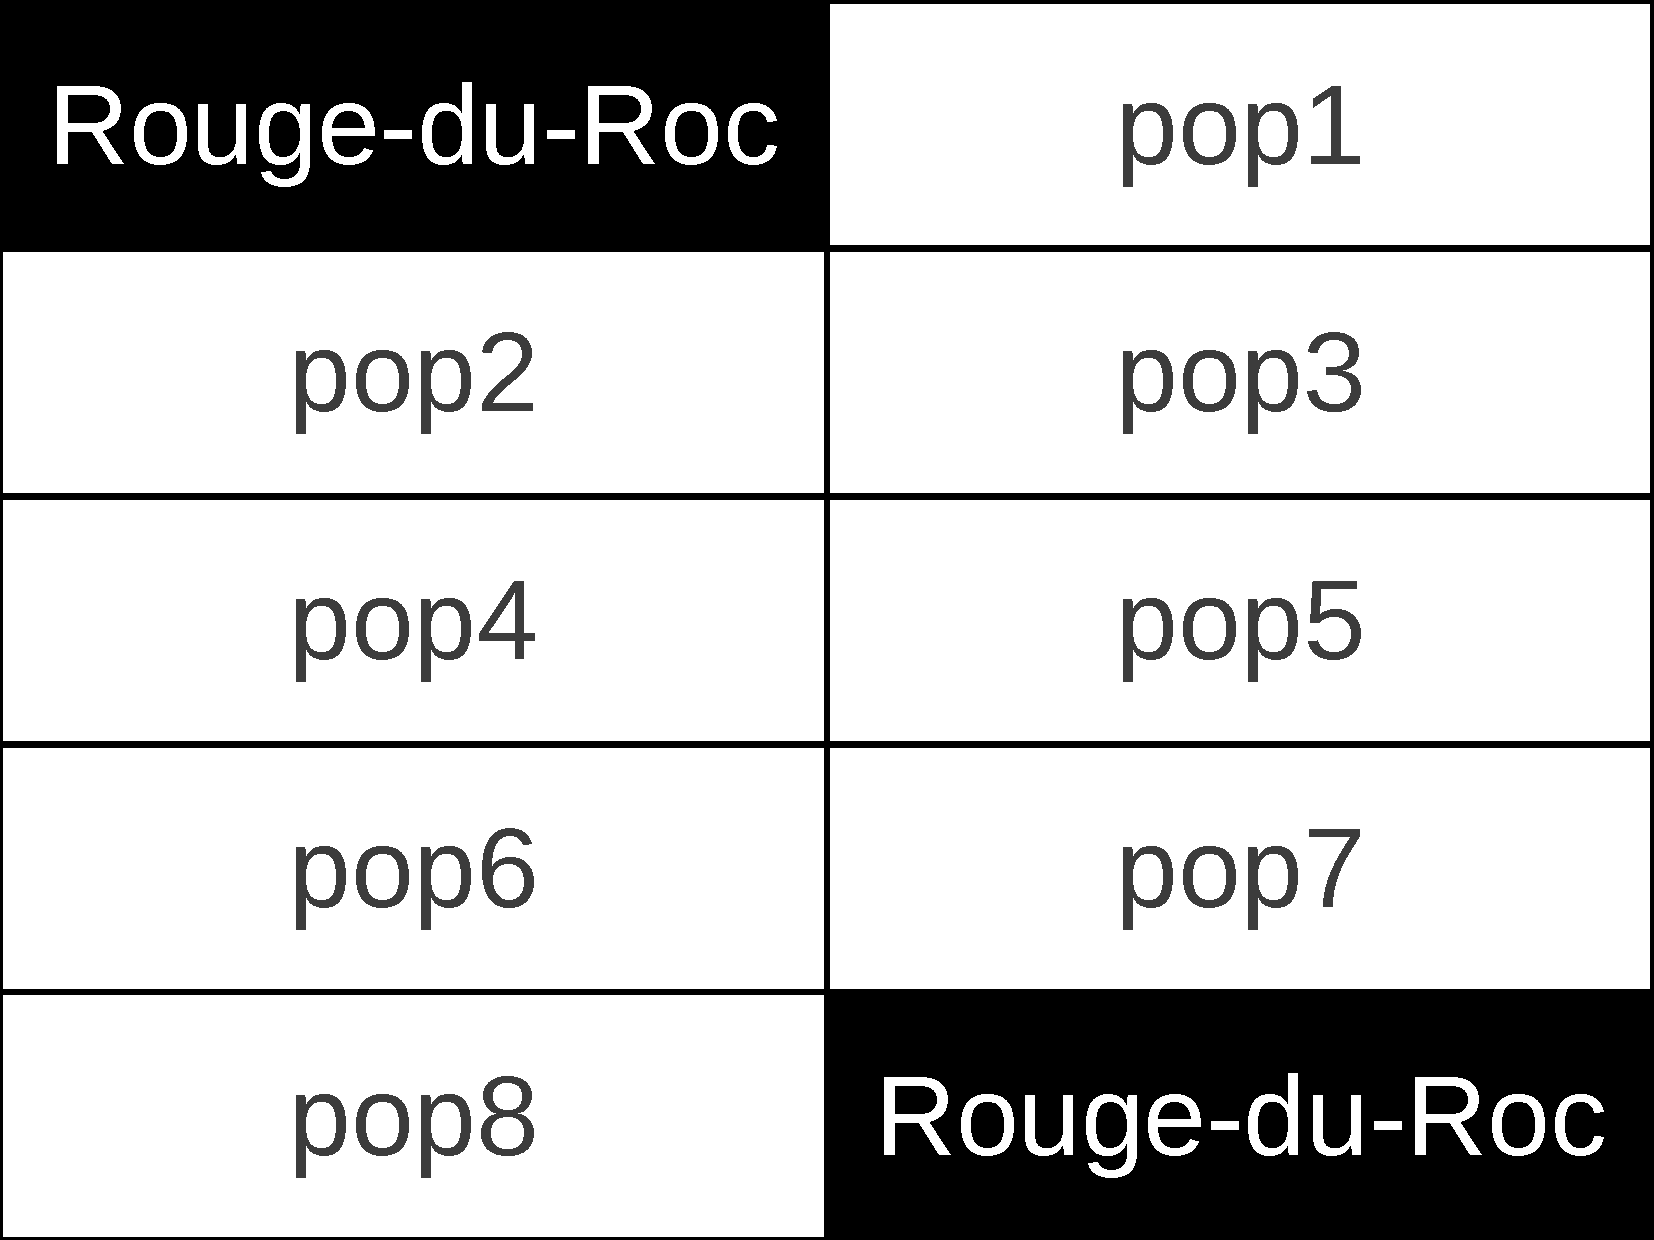
\includegraphics[width=.25\textwidth]{plan_FS.pdf}
                        &
                        \vspace{.5cm}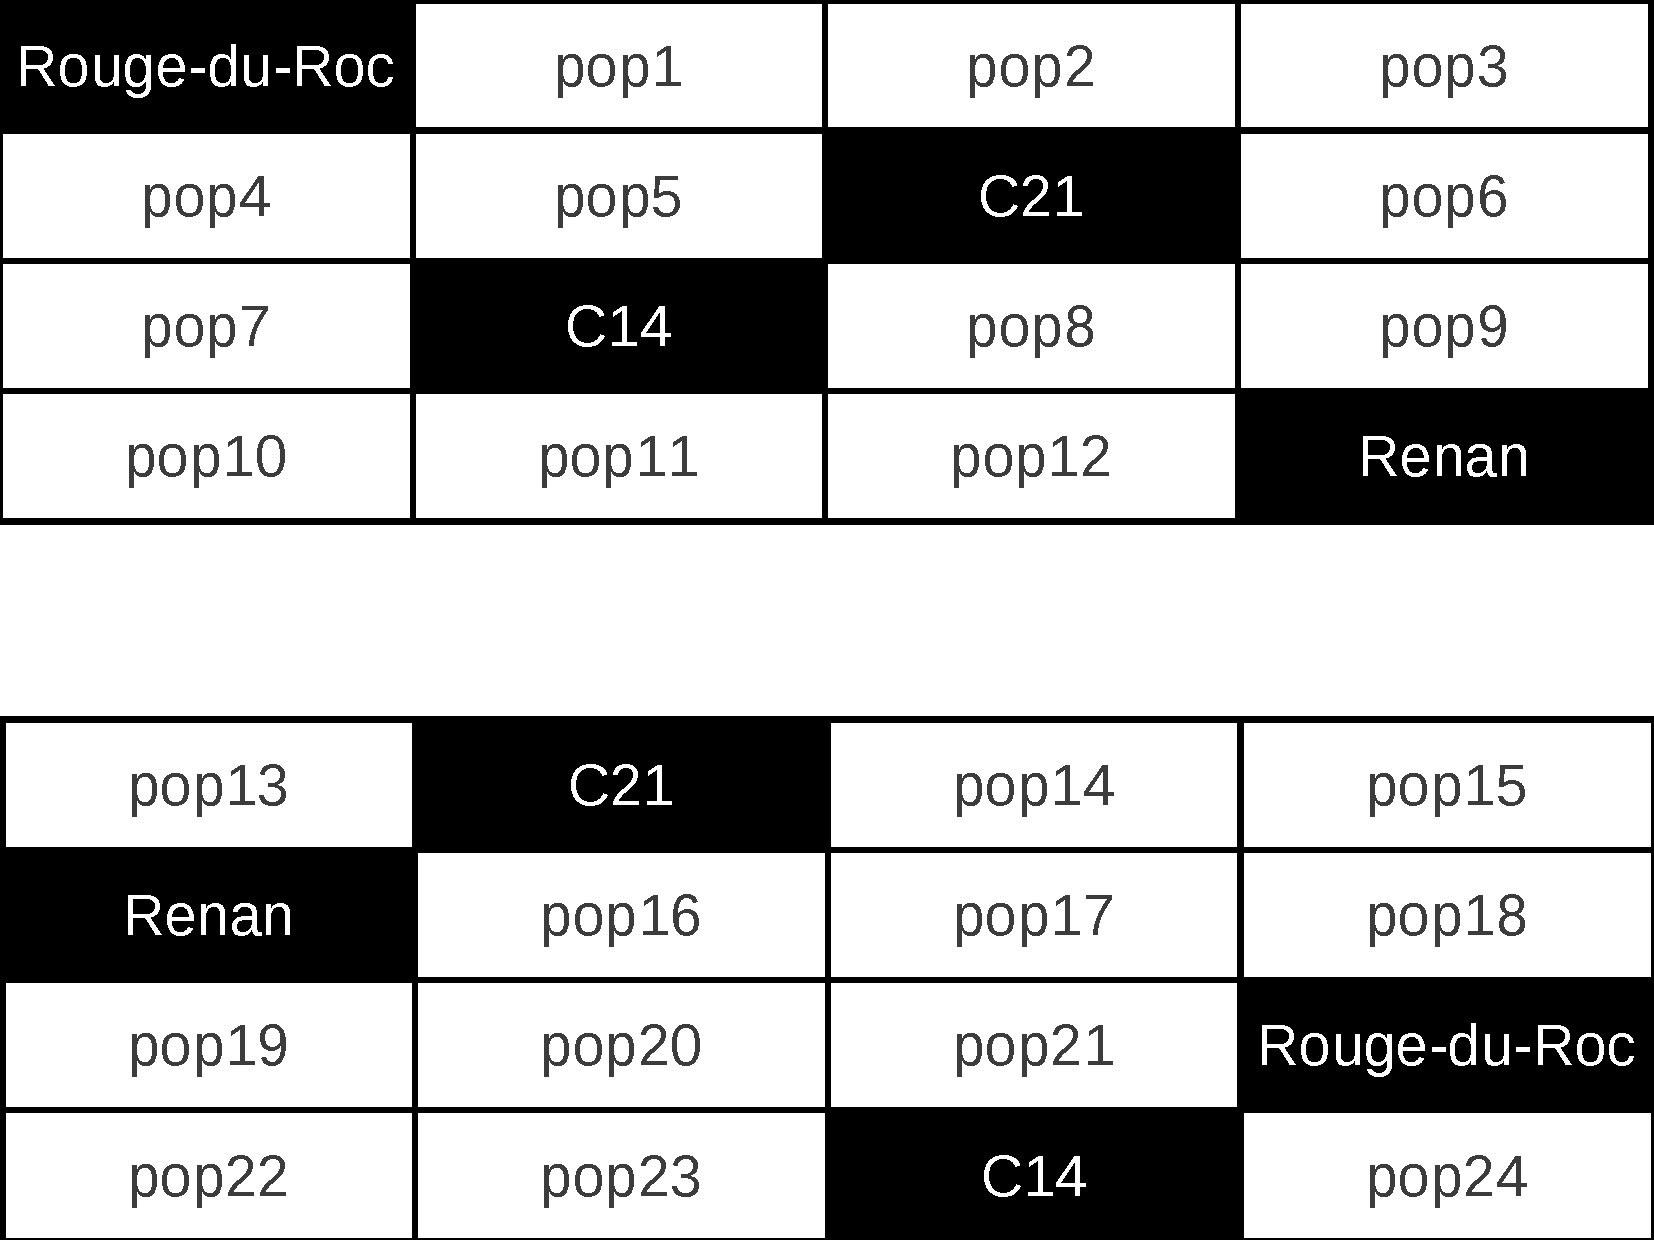
\includegraphics[width=.45\textwidth]{plan_FR.pdf} \\
                        satellite farm & regional farm \\
                        \hline
                \end{tabular}

                \caption{Experimental design of satellite and regional farms. Controls replicated are in black boxes : $Rouge$-$du$-$Roc$, $Renan$, $C14$ and $C21$. pop stands for `tested population'.}
                \label{plan_SF_RF}
        \end{center}
\end{figure}

\begin{itemize}
\item At the \textbf{farm level}, the residual had few degrees of freedom, leading to a poor estimation of the residual variance and to a lack of power for comparing populations.
Hence, model~\ref{model1} was implemented (section~\ref{section_model1}).

\item At the \textbf{network level}, there is a large germplasm $\times$ environment combinaisons that are missing, leading to a poor estimation of germplasm, environment and interaction effects.
Hence, model~\ref{model2} was implemented (section~\ref{section_model2}).

\end{itemize}

These methods are of interest if you have a large data set with a high number of environments and germplasms.
For model \ref{model1}, it gave nice results with more than 20 environment \citep{riviere_hierarchical_2015}.
For model \ref{model2}, it gave nice results with 75 environments and 120 germplasms present in at least two environments (95\% of missing $G \times E$ combinaisons) \citep{riviere_hierarchical_2016}.

This will be further explore in simulation studies.

\subsection{Function relations in \pack}

\pack~is divided into two sets of functions:


\begin{itemize}
\item Hidden functions
\item Used functions
\end{itemize}


In this vignette, we only used examples with used functions.
Nevertheless, hidden functions could be used in other context to answer specific questions.
Figure~\ref{function_relations} displays these functions and their relations.
Table~\ref{function_descriptions} gives a quick description of each function.
You can have more information for each function by typing \texttt{?function\_name} in your \R~session.


\begin{figure}[H]
\begin{center}
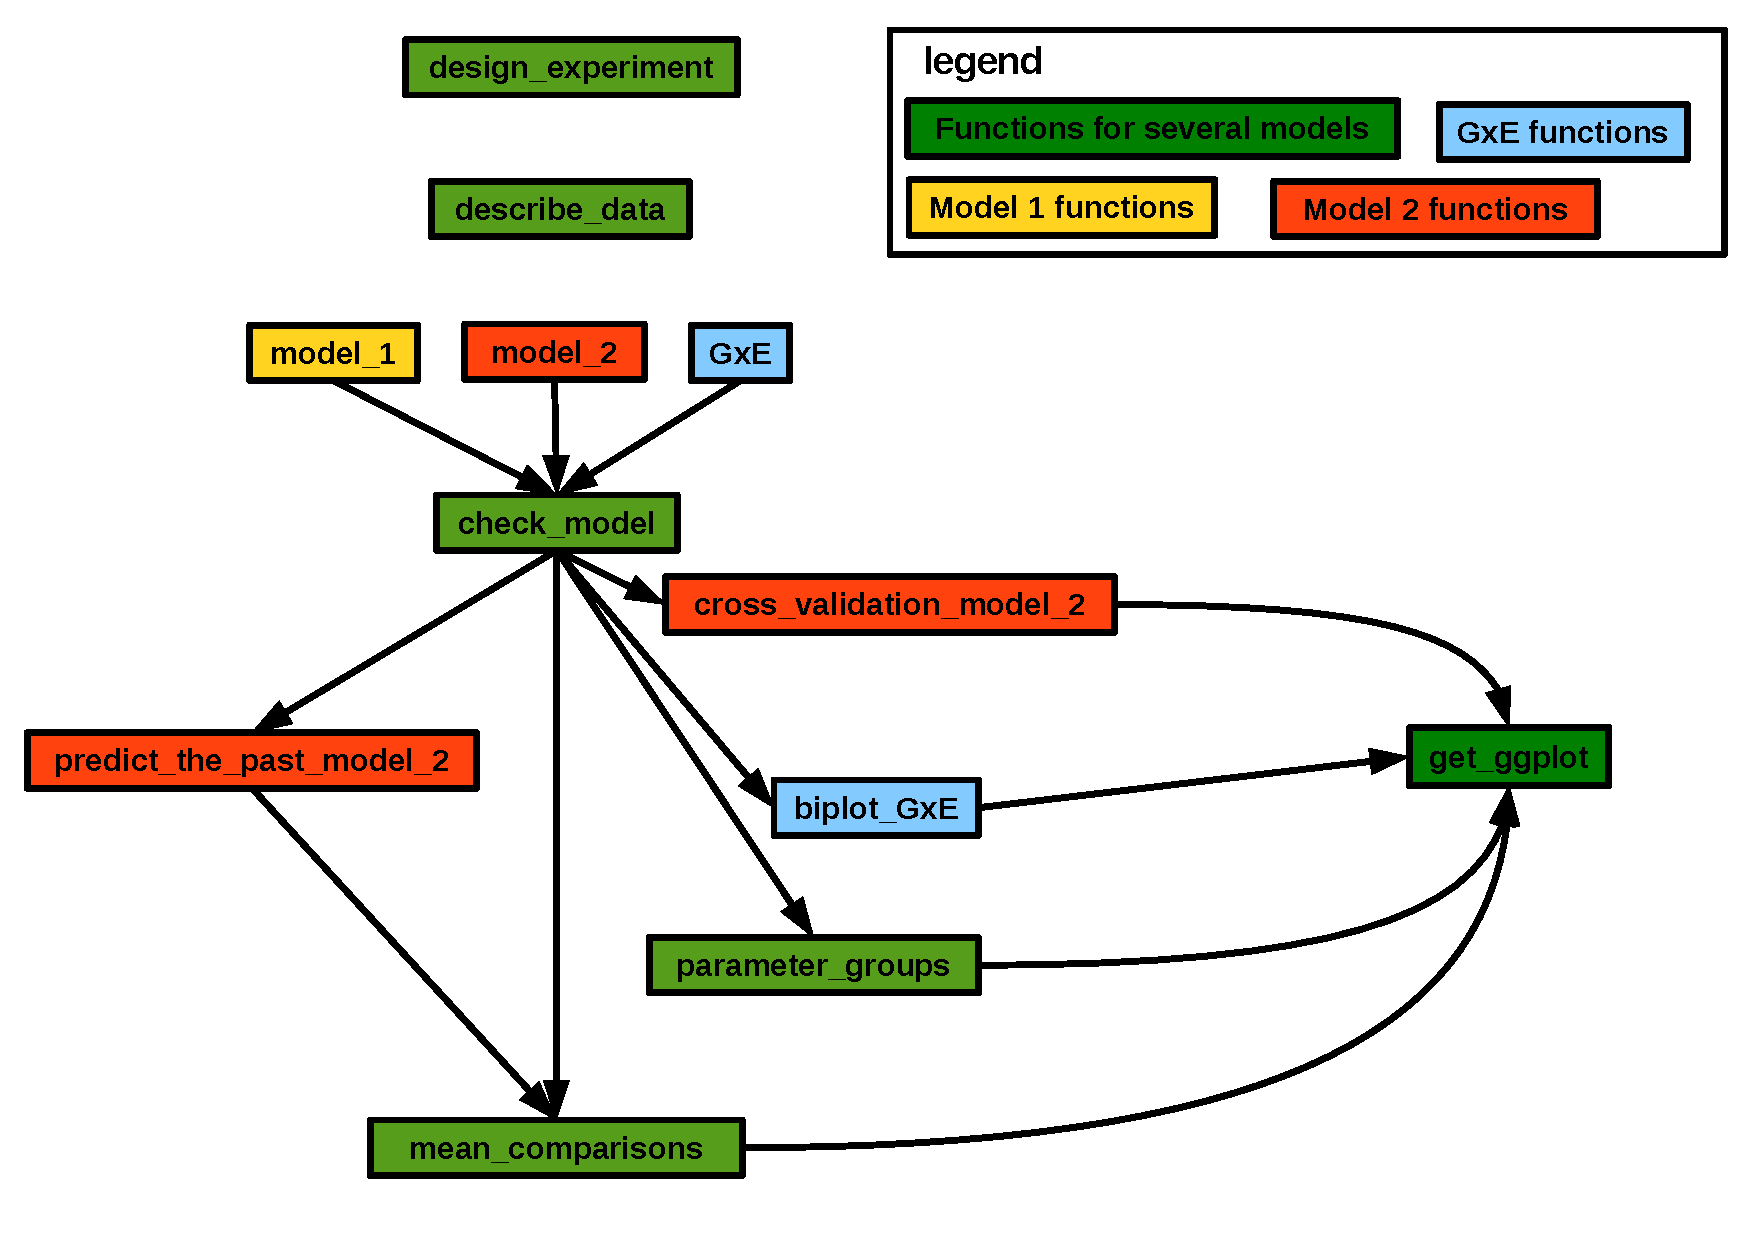
\includegraphics[width=\textwidth]{PBBstats_function_relations}
\end{center}
\caption{Function relations in \pack.
Functions related to model \ref{model1} are in red.
Functions related to model \ref{model2} are in orange.
Functions related to both models are in black.
}
\label{function_relations}
\end{figure}

\begin{table}[t]
\begin{tabular}{cp{.6\textwidth}}

\hline
\textbf{function name} & \textbf{description} \\

\hline
\hline

\texttt{MC} & Run model~\ref{model1} to get mean comparisons (MC) on each environment of the network.\\
\hline

\texttt{FWH} & Run model~\ref{model2} to get main germplasm, environment and sensitivity effects over the network. \\
\hline

\texttt{analyse.outputs} & Check with plots if the model went well based ont the Gelman-Rubin test and plots of posteriors distributions (see section \ref{section_bayes}). It is important to run this step before going ahead in the analysis otherwise you may make mistakes in the interpretation of the results \\
\hline

\texttt{get.mean.comparisons} & Get mean comparisons for a given parameter two by two or to a given threshold based on MCMC outputs \\
\hline

\texttt{get.parameter.groups} & Get groups of parameters based on multivariate analysis \\
\hline

\texttt{cross.validation.FWH} & Run complete cross vlidation with model~\ref{model2} \\
\hline

\texttt{predict.the.past} & Estimate value of a germplasm in an environment based on the FWH model. \\
\hline

\texttt{get.ggplot} & Get ggplot objects to visualize output from the analysis \\
\hline

\hline


\texttt{get.env.info} & Get regional farms data and satellite farms data \\
\hline

\texttt{comp.parameters} & Get parameter comparisons two by two or to a given threshold based on MCMC outputs \\
\hline

\texttt{get.significant.groups} & Get significant groups of differences for a set of parameters based on MCMC outputs \\
\hline

\texttt{get.at.least.X.groups} & Get the value of type one error needed to have X groups. \\
\hline


\end{tabular}
\caption{Function descriptions in \pack.}
\label{function_descriptions}
\end{table}




\subsection{Bayesian statistics}
\label{section_bayes}

The analyses performed in \pack~are based on Bayesian statistics.

Bayesian statistics are based on the Bayes theorem:

\begin{displaymath}
Pr(\theta|y) \propto Pr(\theta) Pr(y|\theta)
\end{displaymath}

with 
$Pr(\theta|y)$ the posterior, 
$Pr(y|\theta)$ the likelihood and 
$Pr(\theta)$ the prior.

The parameters' distribution, knowing the data (the posterior), is proportional to the distribution \textit{a  priori} (the prior) $\times$ the information brought by the data (the likelihood).

The more information (i.e. the larger the data set and the better the model fits the data), the less the prior would be of importance.
If the priors equal the posteriors, it means that there is not enough data or the model does not fit the data.


Bayesian inference is based on the posterior distribution of model parameters.
This distribution could not be calculated explicitely for the hierarchical model used in here (see section~\ref{section_model1} and section~\ref{section_model2}) but could be estimated using Markov Chain and Monte Carlo (MCMC) methods.

These methods simulate values of model parameters according to a Markov chain that converges to the posterior distribution of model parameters \citep{robert_bayesian_2001}.

MCMC methods were implemented using \texttt{JAGS} by the \texttt{R} package \texttt{rjags} that performed Gibbs sampling \citep{robert_bayesian_2001}.
Two MCMC chains were run independently to test for convergence using the Gelman-Rubin test.
This test was based on the variance within and between the chains \citep{gelman_inference_1992}.

A burn-in and lots of iterations were needed in the MCMC procedure.
In our case, the burn-in had 1000 iterations, then 100 000 iterations are done by default\footnote{You can change it with the argument \texttt{nb\_iterations} in functions \texttt{MC} and \texttt{FWH}} with a thinning interval of 10 to reduce autocorrelations between samples, so that 10 000 samples were available for inference for each chain by default\footnote{There are \texttt{nb\_iterations}/10 values for each chain. This can be changed with the \texttt{thin} argument of the functions.}.
 
The final distribution of a posterior is the concatenation of the two MCMC chains: 20 000 samples.

